%TC:ignore
\setcounter{table}{0}
\renewcommand{\thetable}{A\arabic{table}}

\begin{appendices}

\section{BitTorrent} \label{app:bittorrent}

Created by Bram Cohen and formalised in 2008, BitTorrent supports P2P filesharing and is commonly used to distribute large files over the Internet with the individual peers, rather than a single server bearing the load and costs \citep{cohen2008} . 

\subsection{Popularity}
Since 2004, BitTorrent has been the most popular P2P protocol (holding 53\% of total P2P traffic) with other competing  protocols such as FastTrack, Gnutella and eDonkey falling in both users and traffic \citep{cachelogictruep2p, cachelogicp2p2}.

\subsection{Overview} \label{app:torrentprocess}

On BitTorrent, users downloading the file are leechers and once the file is complete, seeders, uploading the file to other users in the network. \Glspl{peer} with a particular file are called the `swarm'. Fig.~\ref{fig:architecture} shows an overview of the BitTorrent network during a download.

\begin{figure}[h]
    \centering
    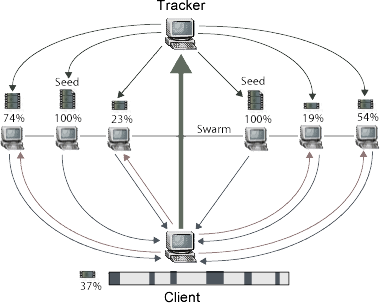
\includegraphics[width=0.6\textwidth]{architecture}
    \caption{Architecture of the BitTorrent network  \citet{history13}}
    \label{fig:architecture}
\end{figure}

\section{Prosecuting a User} \label{app:legaloptions}

\citet{MDE:MDE2634} argues that the usual intent of lawsuits against torrenters is to ``change user behaviour'' in an attempt to discourage users from sharing files on the network and not to recover ``meaningful damages''. ``Discouraging users'' has been key since Chan Nai-ming, the first person to be convicted of piracy, who was sentenced to 3 months imprisonment \citep{bigcrook07}.

In order to prosecute an individual user of the BitTorrent network, the prosecution must present evidence of that user using the network to download or share copyrighted works without permission of the copyright holder.

\subsection{Downloading}
It is difficult to track a download occurring due to the distributed nature of the P2P network.
Pieces of the file come from many different locations at once, no one server provides the whole file so it's hard to link the connections to one instance of infringement. Additionally, because the file is split into many pieces, it is problematic to prove each piece is a part of a copyrighted work. Legally, even if a download is witnessed it must be proven that the downloader is deliberately infringing copyright.

\subsection{Sharing}
Demonstrating sharing is technically simple. A user would simply need to request a particular \textit{.torrent} from the \gls{swarm} and log those listed as peers who have copies of the file available for download. This would also serve as a legal demonstration of the intent to distribute copyright-protected material.

\section{Prosecuting a Tracker}
There have been several successful, high profile cases against the \glspl{tracker} that index the copyrighted works to make them available to the general downloader \citep{fungvsmpaa}.
Commonly in the United Kingdom, the legal responsibility now falls against the Internet Service Provider's (\gls{isp}'s)  that provide access to the \glspl{tracker}, rather than the \glspl{tracker} themselves \citep{bpivsukisps}. Due to the multinational nature of the Internet, there is often complication as to with whom jurisdiction falls.

\section{BPI vs UK ISP's} \label{app:bpiVtpb}

Dramatico Entertainment Limited, Emi Records Limited, Mercury Records Limited, Polydor Limited, Rough Trade Records Limited,Sony Music Entertainment UK Limited, Virgin Records Limited, Warner Music Uk Limited, and 679 Recordings Limited vs. British Sky Broadcasting Limited, British Telecommunications Plc, Everything Everywhere Limited, Talktalk Telecom Group Plc, Telefonica UK Limited, and Virgin Media Limited.

\subsection{Charges}
The court found the users guilty on two counts. Firstly, copying as defined in section 17 of the Copyright, Designs and Patents Act (CDPA) \citep{cdpa}; arguing that by selecting a torrent, a user is willing infringing copyright and highlighting that during download the file contents are copied to the user's computer. Secondly, ``communicating to the public'' as defined in section 20 of CDPA, citing  ``communication to the public must be interpreted broadly'' (\citet[47.]{courtofjustice2012} as cited in \citet{bpivsukisps}) in order to apply it to the Internet and that ``at least 15\% of the sample records were being shared'' \citep{bpivsukisps}.

The court found the operators of The Pirate Bay guilty of authorisation or assisting the infringement; pointing out that the operators go far beyond enabling and assisting the copyright infringement, 
 they ``sanction, approve and countenance'' and that they are ``providing means to infringe, encouraging infringement and taking no steps to prevent'' it \citep{bpivsukisps}.

\section{HADOPI} \label{app:hadopi}

In an attempt to limit the spread of piracy throughout France, the French government created a dedicated department agency, the High Authority for Transmission of Creative Works and Copyright Protection on the Interne, to address this problem and to increase sales in the French media industry.
This department was mandated to identify and prosecute French Internet users who had been identified as sharing or downloading copyrighted materials using a three strike system, starting with education and ending in prosecution, disconnection from the Internet and fine's.
However, after enforcing this law and sending out over a million warnings, research found that increased sales stemmed from the education component of the `HADOPI law' \citep{danaher2012hadopi}, and not the prosecution element as expected. This suggested that prosecution of copyright infringers did not deter people from digital piracy \citep{peoples2012hadopi}. 

In May 2013 a government report recommended the removal of the law \citep{lescure2013}. In July 2013 the French government abolished the law choosing to target `commercial piracy' and `sites that profit from pirated material' \citet{guardian2013hadopi}.

\section{Avoiding the Blocks} \label{app:avoidingblocks}

It is easy to avoid blocks, anybody could do it following a tutorial, particularly with the rapid increase of tutorials and proxies following a block. For example simply typing `pirate bay proxy' into Google returns hundreds of websites designed to avoid the blocks.

The operators can also perform one of many tricks to mitigate the blocks due to the technical way that the blocks are enforced, including change of a servers IP address and use of a different domain \citep{piratebaylegal}.

\section{Tables}

\begin{table}[H]
\centering
\begin{tabular}{m{2cm}m{3cm}m{7cm}m{2cm}}
\textbf{By} & \textbf{Against} & \textbf{Reason} & \textbf{Date} \\
\hline
BPI &   The Pirate Bay            & Authorisation of copyright infringement & May 2012 \\
FACT-UK & \begin{tabular}[l]{@{}l@{}}Fenopy\\ H33t\\ KickassTorrents\end{tabular}                                                                                & Enabling mass access to infringing content        & March 2013  \\
MPAA & Movie2k                  & \textit{Court order not published}        & May 2013  \\
MPAA & Download For All         & \textit{Court order not published}        & May 2013  \\
FACT-UK \& MPAA & EZTV          & Communication to the public (of copyrighted content)       & July 2013 \\
PPL \& BPI & \begin{tabular}[l]{@{}l@{}}
1337x\\
Abmp3\\
Bit Snoop\\
BeeMPS\\
Bomb-Mp3e\\ 
Mp3World\\ 
ExtraTorrent\\ 
File Crop\\ 
FilesTube\\ 
Monova\\ Mp3 Juices\\ Mp3lemon\\ Mp3 Raid\\ Mp3 Skull\\ New Album Releases\\ Rapid Library\\ Torrent Crazy\\ Torrent Downloads\\ Torrent Hound\\ Torrent Reactor\\ Torrentz
\end{tabular}                   & Commercially exploiting music without a licence & October 2013  \\
FACT-UK & YIFY Torrents                   & Communication to the public (of copyrighted content) & November 2013 \\
\end{tabular}

\caption{UK Court ordered blocks against file sharing websites \citep{emivsisp, footballvseztv, skycopyright, bbcblock21, bbcblocks2}}
\label{table:courtorders}
\end{table}

\end{appendices}
%TC:endignore